\documentclass[1p]{elsarticle_modified}
%\bibliographystyle{elsarticle-num}

%\usepackage[colorlinks]{hyperref}
%\usepackage{abbrmath_seonhwa} %\Abb, \Ascr, \Acal ,\Abf, \Afrak
\usepackage{amsfonts}
\usepackage{amssymb}
\usepackage{amsmath}
\usepackage{amsthm}
\usepackage{scalefnt}
\usepackage{amsbsy}
\usepackage{kotex}
\usepackage{caption}
\usepackage{subfig}
\usepackage{color}
\usepackage{graphicx}
\usepackage{xcolor} %% white, black, red, green, blue, cyan, magenta, yellow
\usepackage{float}
\usepackage{setspace}
\usepackage{hyperref}

\usepackage{tikz}
\usetikzlibrary{arrows}

\usepackage{multirow}
\usepackage{array} % fixed length table
\usepackage{hhline}

%%%%%%%%%%%%%%%%%%%%%
\makeatletter
\renewcommand*\env@matrix[1][\arraystretch]{%
	\edef\arraystretch{#1}%
	\hskip -\arraycolsep
	\let\@ifnextchar\new@ifnextchar
	\array{*\c@MaxMatrixCols c}}
\makeatother %https://tex.stackexchange.com/questions/14071/how-can-i-increase-the-line-spacing-in-a-matrix
%%%%%%%%%%%%%%%

\usepackage[normalem]{ulem}

\newcommand{\msout}[1]{\ifmmode\text{\sout{\ensuremath{#1}}}\else\sout{#1}\fi}
%SOURCE: \msout is \stkout macro in https://tex.stackexchange.com/questions/20609/strikeout-in-math-mode

\newcommand{\cancel}[1]{
	\ifmmode
	{\color{red}\msout{#1}}
	\else
	{\color{red}\sout{#1}}
	\fi
}

\newcommand{\add}[1]{
	{\color{blue}\uwave{#1}}
}

\newcommand{\replace}[2]{
	\ifmmode
	{\color{red}\msout{#1}}{\color{blue}\uwave{#2}}
	\else
	{\color{red}\sout{#1}}{\color{blue}\uwave{#2}}
	\fi
}

\newcommand{\Sol}{\mathcal{S}} %segment
\newcommand{\D}{D} %diagram
\newcommand{\A}{\mathcal{A}} %arc


%%%%%%%%%%%%%%%%%%%%%%%%%%%%%5 test

\def\sl{\operatorname{\textup{SL}}(2,\Cbb)}
\def\psl{\operatorname{\textup{PSL}}(2,\Cbb)}
\def\quan{\mkern 1mu \triangleright \mkern 1mu}

\theoremstyle{definition}
\newtheorem{thm}{Theorem}[section]
\newtheorem{prop}[thm]{Proposition}
\newtheorem{lem}[thm]{Lemma}
\newtheorem{ques}[thm]{Question}
\newtheorem{cor}[thm]{Corollary}
\newtheorem{defn}[thm]{Definition}
\newtheorem{exam}[thm]{Example}
\newtheorem{rmk}[thm]{Remark}
\newtheorem{alg}[thm]{Algorithm}

\newcommand{\I}{\sqrt{-1}}
\begin{document}

%\begin{frontmatter}
%
%\title{Boundary parabolic representations of knots up to 8 crossings}
%
%%% Group authors per affiliation:
%\author{Yunhi Cho} 
%\address{Department of Mathematics, University of Seoul, Seoul, Korea}
%\ead{yhcho@uos.ac.kr}
%
%
%\author{Seonhwa Kim} %\fnref{s_kim}}
%\address{Center for Geometry and Physics, Institute for Basic Science, Pohang, 37673, Korea}
%\ead{ryeona17@ibs.re.kr}
%
%\author{Hyuk Kim}
%\address{Department of Mathematical Sciences, Seoul National University, Seoul 08826, Korea}
%\ead{hyukkim@snu.ac.kr}
%
%\author{Seokbeom Yoon}
%\address{Department of Mathematical Sciences, Seoul National University, Seoul, 08826,  Korea}
%\ead{sbyoon15@snu.ac.kr}
%
%\begin{abstract}
%We find all boundary parabolic representation of knots up to 8 crossings.
%
%\end{abstract}
%\begin{keyword}
%    \MSC[2010] 57M25 
%\end{keyword}
%
%\end{frontmatter}

%\linenumbers
%\tableofcontents
%
\newcommand\colored[1]{\textcolor{white}{\rule[-0.35ex]{0.8em}{1.4ex}}\kern-0.8em\color{red} #1}%
%\newcommand\colored[1]{\textcolor{white}{ #1}\kern-2.17ex	\textcolor{white}{ #1}\kern-1.81ex	\textcolor{white}{ #1}\kern-2.15ex\color{red}#1	}

{\Large $\underline{11a_{81}~(K11a_{81})}$}

\setlength{\tabcolsep}{10pt}
\renewcommand{\arraystretch}{1.6}
\vspace{1cm}\begin{tabular}{m{100pt}>{\centering\arraybackslash}m{274pt}}
\multirow{5}{120pt}{
	\centering
	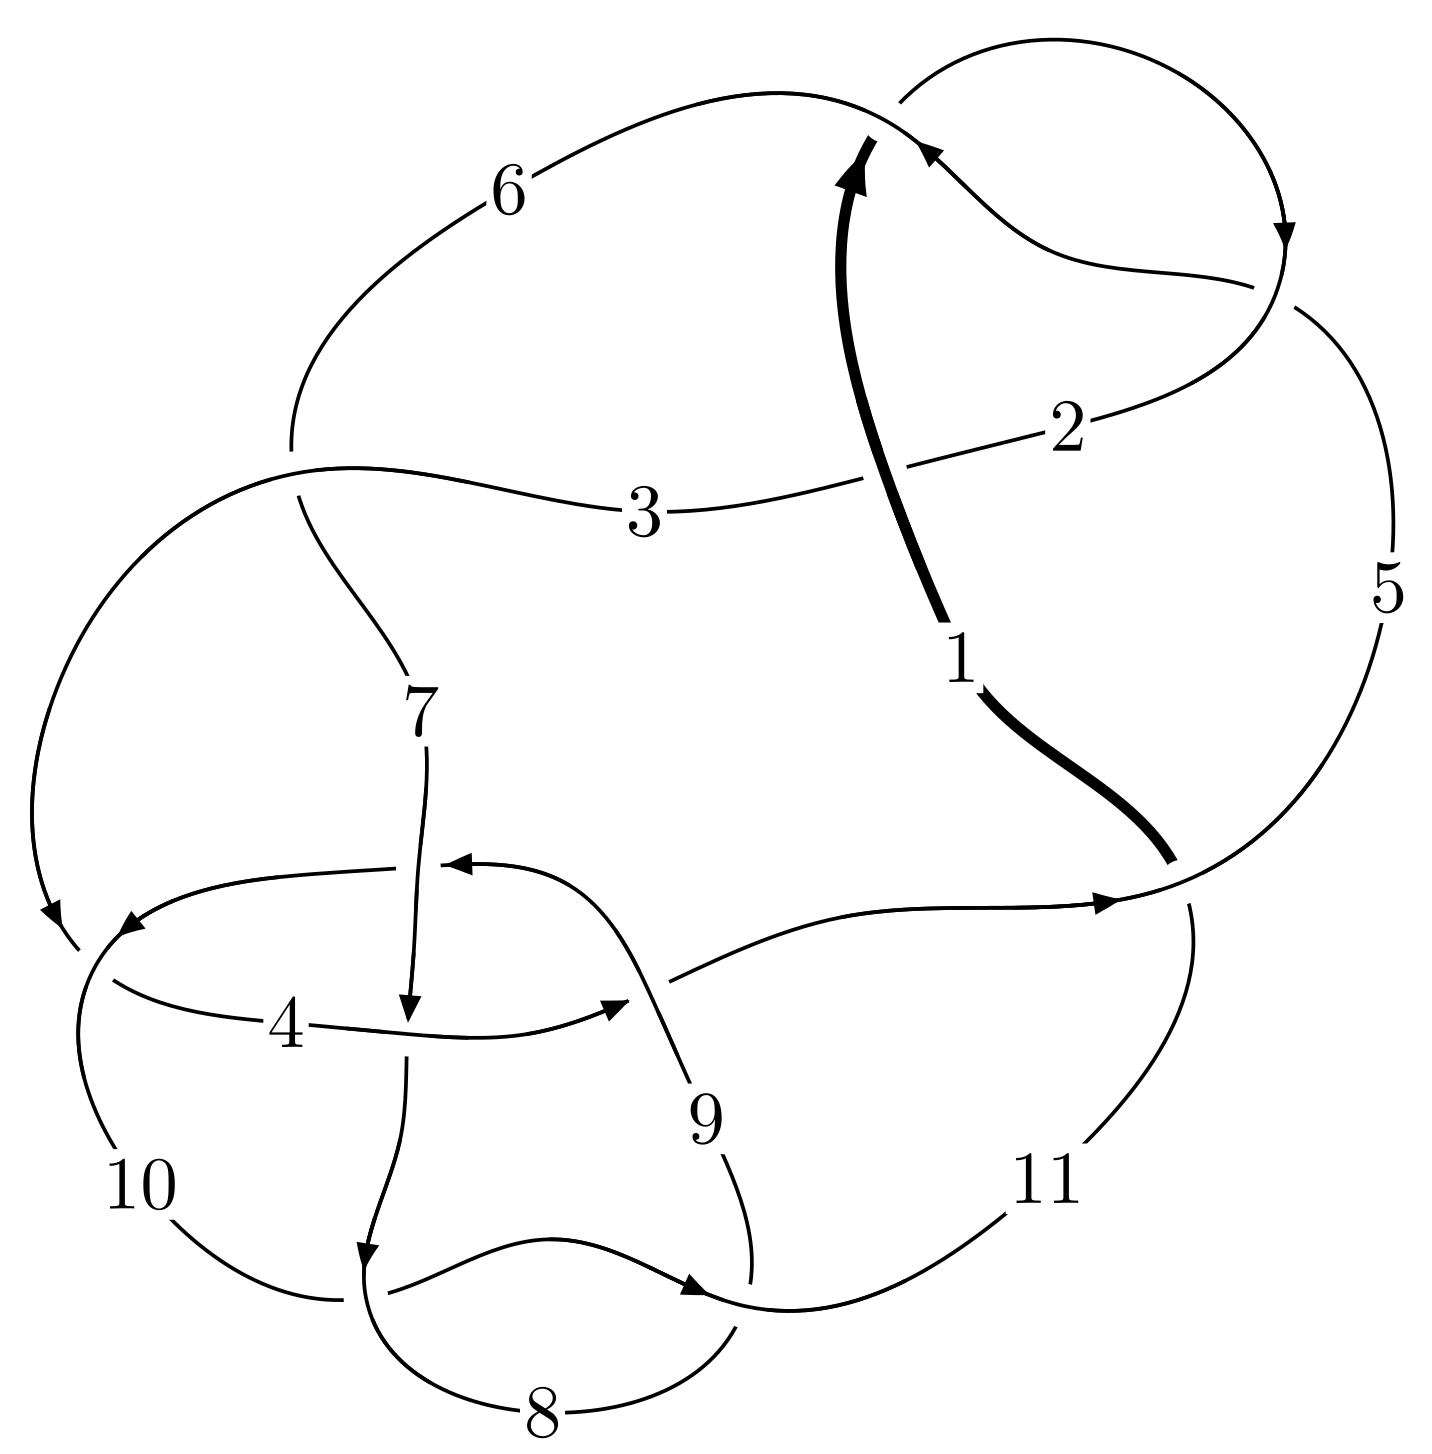
\includegraphics[width=112pt]{../../../GIT/diagram.site/Diagrams/png/330_11a_81.png}\\
\ \ \ A knot diagram\footnotemark}&
\allowdisplaybreaks
\textbf{Linearized knot diagam} \\
\cline{2-2}
 &
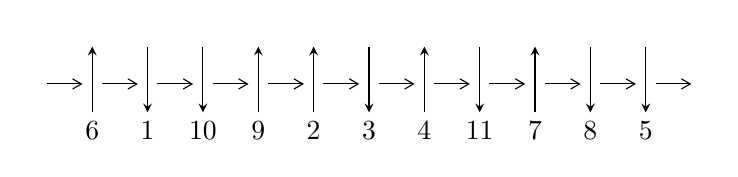
\begin{tikzpicture}[x=20pt, y=17pt]
	% nodes
	\node (C0) at (0, 0) {};
	\node (C1) at (1, 0) {};
	\node (C1U) at (1, +1) {};
	\node (C1D) at (1, -1) {6};

	\node (C2) at (2, 0) {};
	\node (C2U) at (2, +1) {};
	\node (C2D) at (2, -1) {1};

	\node (C3) at (3, 0) {};
	\node (C3U) at (3, +1) {};
	\node (C3D) at (3, -1) {10};

	\node (C4) at (4, 0) {};
	\node (C4U) at (4, +1) {};
	\node (C4D) at (4, -1) {9};

	\node (C5) at (5, 0) {};
	\node (C5U) at (5, +1) {};
	\node (C5D) at (5, -1) {2};

	\node (C6) at (6, 0) {};
	\node (C6U) at (6, +1) {};
	\node (C6D) at (6, -1) {3};

	\node (C7) at (7, 0) {};
	\node (C7U) at (7, +1) {};
	\node (C7D) at (7, -1) {4};

	\node (C8) at (8, 0) {};
	\node (C8U) at (8, +1) {};
	\node (C8D) at (8, -1) {11};

	\node (C9) at (9, 0) {};
	\node (C9U) at (9, +1) {};
	\node (C9D) at (9, -1) {7};

	\node (C10) at (10, 0) {};
	\node (C10U) at (10, +1) {};
	\node (C10D) at (10, -1) {8};

	\node (C11) at (11, 0) {};
	\node (C11U) at (11, +1) {};
	\node (C11D) at (11, -1) {5};
	\node (C12) at (12, 0) {};

	% arrows
	\draw[->,>={angle 60}]
	(C0) edge (C1) (C1) edge (C2) (C2) edge (C3) (C3) edge (C4) (C4) edge (C5) (C5) edge (C6) (C6) edge (C7) (C7) edge (C8) (C8) edge (C9) (C9) edge (C10) (C10) edge (C11) (C11) edge (C12) ;	\draw[->,>=stealth]
	(C1D) edge (C1U) (C2U) edge (C2D) (C3U) edge (C3D) (C4D) edge (C4U) (C5D) edge (C5U) (C6U) edge (C6D) (C7D) edge (C7U) (C8U) edge (C8D) (C9D) edge (C9U) (C10U) edge (C10D) (C11U) edge (C11D) ;
	\end{tikzpicture} \\
\hhline{~~} \\& 
\textbf{Solving Sequence} \\ \cline{2-2} 
 &
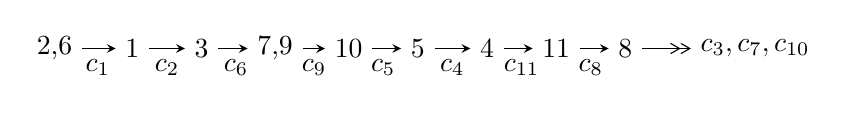
\begin{tikzpicture}[x=25pt, y=7pt]
	% node
	\node (A0) at (-1/8, 0) {2,6};
	\node (A1) at (1, 0) {1};
	\node (A2) at (2, 0) {3};
	\node (A3) at (49/16, 0) {7,9};
	\node (A4) at (33/8, 0) {10};
	\node (A5) at (41/8, 0) {5};
	\node (A6) at (49/8, 0) {4};
	\node (A7) at (57/8, 0) {11};
	\node (A8) at (65/8, 0) {8};
	\node (C1) at (1/2, -1) {$c_{1}$};
	\node (C2) at (3/2, -1) {$c_{2}$};
	\node (C3) at (5/2, -1) {$c_{6}$};
	\node (C4) at (29/8, -1) {$c_{9}$};
	\node (C5) at (37/8, -1) {$c_{5}$};
	\node (C6) at (45/8, -1) {$c_{4}$};
	\node (C7) at (53/8, -1) {$c_{11}$};
	\node (C8) at (61/8, -1) {$c_{8}$};
	\node (A9) at (10, 0) {$c_{3},c_{7},c_{10}$};

	% edge
	\draw[->,>=stealth]	
	(A0) edge (A1) (A1) edge (A2) (A2) edge (A3) (A3) edge (A4) (A4) edge (A5) (A5) edge (A6) (A6) edge (A7) (A7) edge (A8) ;
	\draw[->>,>={angle 60}]	
	(A8) edge (A9);
\end{tikzpicture} \\ 

\end{tabular} \\

\footnotetext{
The image of knot diagram is generated by the software ``\textbf{Draw programme}" developed by Andrew Bartholomew(\url{http://www.layer8.co.uk/maths/draw/index.htm\#Running-draw}), where we modified some parts for our purpose(\url{https://github.com/CATsTAILs/LinksPainter}).
}\phantom \\ \newline 
\centering \textbf{Ideals for irreducible components\footnotemark of $X_{\text{par}}$} 
 
\begin{align*}
I^u_{1}&=\langle 
1.12437\times10^{21} u^{64}+2.08104\times10^{21} u^{63}+\cdots+3.92161\times10^{20} b-9.56908\times10^{20},\\
\phantom{I^u_{1}}&\phantom{= \langle  }6.77960\times10^{19} u^{64}-7.94718\times10^{20} u^{63}+\cdots+3.92161\times10^{20} a+1.89541\times10^{21},\;u^{65}+2 u^{64}+\cdots+u-1\rangle \\
I^u_{2}&=\langle 
b+u,\;a- u-1,\;u^2+u+1\rangle \\
\\
\end{align*}
\raggedright * 2 irreducible components of $\dim_{\mathbb{C}}=0$, with total 67 representations.\\
\footnotetext{All coefficients of polynomials are rational numbers. But the coefficients are sometimes approximated in decimal forms when there is not enough margin.}
\newpage
\renewcommand{\arraystretch}{1}
\centering \section*{I. $I^u_{1}= \langle 1.12\times10^{21} u^{64}+2.08\times10^{21} u^{63}+\cdots+3.92\times10^{20} b-9.57\times10^{20},\;6.78\times10^{19} u^{64}-7.95\times10^{20} u^{63}+\cdots+3.92\times10^{20} a+1.90\times10^{21},\;u^{65}+2 u^{64}+\cdots+u-1 \rangle$}
\flushleft \textbf{(i) Arc colorings}\\
\begin{tabular}{m{7pt} m{180pt} m{7pt} m{180pt} }
\flushright $a_{2}=$&$\begin{pmatrix}1\\0\end{pmatrix}$ \\
\flushright $a_{6}=$&$\begin{pmatrix}0\\u\end{pmatrix}$ \\
\flushright $a_{1}=$&$\begin{pmatrix}1\\u^2\end{pmatrix}$ \\
\flushright $a_{3}=$&$\begin{pmatrix}u^2+1\\u^4\end{pmatrix}$ \\
\flushright $a_{7}=$&$\begin{pmatrix}- u^5-2 u^3- u\\- u^7- u^5+u\end{pmatrix}$ \\
\flushright $a_{9}=$&$\begin{pmatrix}-0.172878 u^{64}+2.02651 u^{63}+\cdots+2.31811 u-4.83325\\-2.86712 u^{64}-5.30659 u^{63}+\cdots+1.95308 u+2.44009\end{pmatrix}$ \\
\flushright $a_{10}=$&$\begin{pmatrix}-0.142247 u^{64}+2.05786 u^{63}+\cdots+1.94975 u-4.74893\\-2.69775 u^{64}-4.93896 u^{63}+\cdots+2.26672 u+2.24110\end{pmatrix}$ \\
\flushright $a_{5}=$&$\begin{pmatrix}- u\\u\end{pmatrix}$ \\
\flushright $a_{4}=$&$\begin{pmatrix}5.04000 u^{64}+5.88259 u^{63}+\cdots-11.8961 u+0.0715256\\0.371835 u^{64}+4.36917 u^{63}+\cdots+11.7089 u-4.79741\end{pmatrix}$ \\
\flushright $a_{11}=$&$\begin{pmatrix}u^4+u^2+1\\- u^4\end{pmatrix}$ \\
\flushright $a_{8}=$&$\begin{pmatrix}-0.206126 u^{64}+1.99373 u^{63}+\cdots+3.07367 u-4.01687\\-3.03387 u^{64}-5.47353 u^{63}+\cdots+2.13727 u+2.43980\end{pmatrix}$\\ \flushright $a_{8}=$&$\begin{pmatrix}-0.206126 u^{64}+1.99373 u^{63}+\cdots+3.07367 u-4.01687\\-3.03387 u^{64}-5.47353 u^{63}+\cdots+2.13727 u+2.43980\end{pmatrix}$\\&\end{tabular}
\flushleft \textbf{(ii) Obstruction class $= -1$}\\~\\
\flushleft \textbf{(iii) Cusp Shapes $= -\frac{3365010802379045894269}{392161237007130374129} u^{64}-\frac{314262698830792944879}{392161237007130374129} u^{63}+\cdots+\frac{15377811800569051171877}{392161237007130374129} u-\frac{7348835260697976503736}{392161237007130374129}$}\\~\\
\newpage\renewcommand{\arraystretch}{1}
\flushleft \textbf{(iv) u-Polynomials at the component}\newline \\
\begin{tabular}{m{50pt}|m{274pt}}
Crossings & \hspace{64pt}u-Polynomials at each crossing \\
\hline $$\begin{aligned}c_{1},c_{5}\end{aligned}$$&$\begin{aligned}
&u^{65}-2 u^{64}+\cdots+u+1
\end{aligned}$\\
\hline $$\begin{aligned}c_{2}\end{aligned}$$&$\begin{aligned}
&u^{65}+36 u^{64}+\cdots-5 u-1
\end{aligned}$\\
\hline $$\begin{aligned}c_{3}\end{aligned}$$&$\begin{aligned}
&u^{65}+2 u^{64}+\cdots-77 u-209
\end{aligned}$\\
\hline $$\begin{aligned}c_{4}\end{aligned}$$&$\begin{aligned}
&u^{65}-14 u^{63}+\cdots-51079 u-9713
\end{aligned}$\\
\hline $$\begin{aligned}c_{6},c_{11}\end{aligned}$$&$\begin{aligned}
&u^{65}+2 u^{64}+\cdots-27 u+17
\end{aligned}$\\
\hline $$\begin{aligned}c_{7}\end{aligned}$$&$\begin{aligned}
&u^{65}-2 u^{64}+\cdots+u-1
\end{aligned}$\\
\hline $$\begin{aligned}c_{8},c_{10}\end{aligned}$$&$\begin{aligned}
&u^{65}-3 u^{64}+\cdots-6 u+1
\end{aligned}$\\
\hline $$\begin{aligned}c_{9}\end{aligned}$$&$\begin{aligned}
&u^{65}+11 u^{64}+\cdots-12 u-4
\end{aligned}$\\
\hline
\end{tabular}\\~\\
\newpage\renewcommand{\arraystretch}{1}
\flushleft \textbf{(v) Riley Polynomials at the component}\newline \\
\begin{tabular}{m{50pt}|m{274pt}}
Crossings & \hspace{64pt}Riley Polynomials at each crossing \\
\hline $$\begin{aligned}c_{1},c_{5}\end{aligned}$$&$\begin{aligned}
&y^{65}+36 y^{64}+\cdots-5 y-1
\end{aligned}$\\
\hline $$\begin{aligned}c_{2}\end{aligned}$$&$\begin{aligned}
&y^{65}-12 y^{64}+\cdots-97 y-1
\end{aligned}$\\
\hline $$\begin{aligned}c_{3}\end{aligned}$$&$\begin{aligned}
&y^{65}-80 y^{64}+\cdots+680999 y-43681
\end{aligned}$\\
\hline $$\begin{aligned}c_{4}\end{aligned}$$&$\begin{aligned}
&y^{65}-28 y^{64}+\cdots-2283276729 y-94342369
\end{aligned}$\\
\hline $$\begin{aligned}c_{6},c_{11}\end{aligned}$$&$\begin{aligned}
&y^{65}-60 y^{64}+\cdots-15013 y-289
\end{aligned}$\\
\hline $$\begin{aligned}c_{7}\end{aligned}$$&$\begin{aligned}
&y^{65}+12 y^{64}+\cdots-5 y-1
\end{aligned}$\\
\hline $$\begin{aligned}c_{8},c_{10}\end{aligned}$$&$\begin{aligned}
&y^{65}-51 y^{64}+\cdots-94 y-1
\end{aligned}$\\
\hline $$\begin{aligned}c_{9}\end{aligned}$$&$\begin{aligned}
&y^{65}+15 y^{64}+\cdots-152 y-16
\end{aligned}$\\
\hline
\end{tabular}\\~\\
\newpage\flushleft \textbf{(vi) Complex Volumes and Cusp Shapes}
$$\begin{array}{c|c|c}  
\text{Solutions to }I^u_{1}& \I (\text{vol} + \sqrt{-1}CS) & \text{Cusp shape}\\
 \hline 
\begin{aligned}
u &= \phantom{-}0.255209 + 0.948908 I \\
a &= -0.99928 + 1.01479 I \\
b &= \phantom{-}2.04192 - 0.64047 I\end{aligned}
 & -4.38791 + 0.83519 I & -11.90532 - 1.80779 I \\ \hline\begin{aligned}
u &= \phantom{-}0.255209 - 0.948908 I \\
a &= -0.99928 - 1.01479 I \\
b &= \phantom{-}2.04192 + 0.64047 I\end{aligned}
 & -4.38791 - 0.83519 I & -11.90532 + 1.80779 I \\ \hline\begin{aligned}
u &= \phantom{-}0.379172 + 0.954880 I \\
a &= \phantom{-}0.44986 + 1.99487 I \\
b &= -0.95093 - 2.01516 I\end{aligned}
 & -3.54308 + 4.03035 I & -8.72949 - 8.88482 I \\ \hline\begin{aligned}
u &= \phantom{-}0.379172 - 0.954880 I \\
a &= \phantom{-}0.44986 - 1.99487 I \\
b &= -0.95093 + 2.01516 I\end{aligned}
 & -3.54308 - 4.03035 I & -8.72949 + 8.88482 I \\ \hline\begin{aligned}
u &= \phantom{-}0.484262 + 0.914397 I \\
a &= \phantom{-}1.118230 + 0.362011 I \\
b &= -2.04011 - 0.02854 I\end{aligned}
 & \phantom{-}0.85073 + 5.73380 I & \phantom{-0.000000 } 0. - 9.30698 I \\ \hline\begin{aligned}
u &= \phantom{-}0.484262 - 0.914397 I \\
a &= \phantom{-}1.118230 - 0.362011 I \\
b &= -2.04011 + 0.02854 I\end{aligned}
 & \phantom{-}0.85073 - 5.73380 I & \phantom{-0.000000 -}0. + 9.30698 I \\ \hline\begin{aligned}
u &= -0.350482 + 0.867729 I \\
a &= \phantom{-}0.86949 - 2.41938 I \\
b &= -2.39364 - 0.40176 I\end{aligned}
 & -2.05273 - 1.79214 I & -3.9608 - 27.3479 I \\ \hline\begin{aligned}
u &= -0.350482 - 0.867729 I \\
a &= \phantom{-}0.86949 + 2.41938 I \\
b &= -2.39364 + 0.40176 I\end{aligned}
 & -2.05273 + 1.79214 I & -3.9608 + 27.3479 I \\ \hline\begin{aligned}
u &= -0.416907 + 0.814224 I \\
a &= -0.0826608 - 0.0580767 I \\
b &= -0.394803 + 0.423441 I\end{aligned}
 & -0.06086 - 1.78141 I & \phantom{-}0.16593 + 3.65886 I \\ \hline\begin{aligned}
u &= -0.416907 - 0.814224 I \\
a &= -0.0826608 + 0.0580767 I \\
b &= -0.394803 - 0.423441 I\end{aligned}
 & -0.06086 + 1.78141 I & \phantom{-}0.16593 - 3.65886 I\\
 \hline 
 \end{array}$$\newpage$$\begin{array}{c|c|c}  
\text{Solutions to }I^u_{1}& \I (\text{vol} + \sqrt{-1}CS) & \text{Cusp shape}\\
 \hline 
\begin{aligned}
u &= -0.688274 + 0.597046 I \\
a &= \phantom{-}0.937870 + 0.013321 I \\
b &= -0.177796 - 0.445216 I\end{aligned}
 & -1.20524 - 3.66120 I & -3.96415 + 8.51812 I \\ \hline\begin{aligned}
u &= -0.688274 - 0.597046 I \\
a &= \phantom{-}0.937870 - 0.013321 I \\
b &= -0.177796 + 0.445216 I\end{aligned}
 & -1.20524 + 3.66120 I & -3.96415 - 8.51812 I \\ \hline\begin{aligned}
u &= \phantom{-}0.895488 + 0.125785 I \\
a &= -0.09492 + 1.43200 I \\
b &= -0.376735 - 0.287159 I\end{aligned}
 & -7.23534 - 2.53854 I & -7.87268 + 2.81634 I \\ \hline\begin{aligned}
u &= \phantom{-}0.895488 - 0.125785 I \\
a &= -0.09492 - 1.43200 I \\
b &= -0.376735 + 0.287159 I\end{aligned}
 & -7.23534 + 2.53854 I & -7.87268 - 2.81634 I \\ \hline\begin{aligned}
u &= \phantom{-}0.042517 + 0.896108 I \\
a &= -1.233970 - 0.489969 I \\
b &= \phantom{-}1.50275 + 1.00485 I\end{aligned}
 & -1.88737 - 1.49983 I & -7.09909 + 4.37897 I \\ \hline\begin{aligned}
u &= \phantom{-}0.042517 - 0.896108 I \\
a &= -1.233970 + 0.489969 I \\
b &= \phantom{-}1.50275 - 1.00485 I\end{aligned}
 & -1.88737 + 1.49983 I & -7.09909 - 4.37897 I \\ \hline\begin{aligned}
u &= -0.873776 + 0.112840 I \\
a &= -0.53746 - 2.51675 I \\
b &= -0.325555 + 0.658517 I\end{aligned}
 & -7.98517 + 11.01330 I & -4.27925 - 5.99396 I \\ \hline\begin{aligned}
u &= -0.873776 - 0.112840 I \\
a &= -0.53746 + 2.51675 I \\
b &= -0.325555 - 0.658517 I\end{aligned}
 & -7.98517 - 11.01330 I & -4.27925 + 5.99396 I \\ \hline\begin{aligned}
u &= -0.457366 + 1.034950 I \\
a &= -0.505700 + 0.060882 I \\
b &= \phantom{-}0.747461 + 0.669285 I\end{aligned}
 & -0.33001 - 3.05900 I & \phantom{-0.000000 } 0 \\ \hline\begin{aligned}
u &= -0.457366 - 1.034950 I \\
a &= -0.505700 - 0.060882 I \\
b &= \phantom{-}0.747461 - 0.669285 I\end{aligned}
 & -0.33001 + 3.05900 I & \phantom{-0.000000 } 0\\
 \hline 
 \end{array}$$\newpage$$\begin{array}{c|c|c}  
\text{Solutions to }I^u_{1}& \I (\text{vol} + \sqrt{-1}CS) & \text{Cusp shape}\\
 \hline 
\begin{aligned}
u &= \phantom{-}0.571139 + 0.977969 I \\
a &= -0.414828 - 0.730148 I \\
b &= \phantom{-}1.62844 + 0.58978 I\end{aligned}
 & -3.06278 + 10.75520 I & \phantom{-0.000000 } 0 \\ \hline\begin{aligned}
u &= \phantom{-}0.571139 - 0.977969 I \\
a &= -0.414828 + 0.730148 I \\
b &= \phantom{-}1.62844 - 0.58978 I\end{aligned}
 & -3.06278 - 10.75520 I & \phantom{-0.000000 } 0 \\ \hline\begin{aligned}
u &= -0.637047 + 0.936500 I \\
a &= \phantom{-}0.173925 + 0.578410 I \\
b &= \phantom{-}0.317828 - 0.930103 I\end{aligned}
 & -2.16059 - 1.39700 I & \phantom{-0.000000 } 0 \\ \hline\begin{aligned}
u &= -0.637047 - 0.936500 I \\
a &= \phantom{-}0.173925 - 0.578410 I \\
b &= \phantom{-}0.317828 + 0.930103 I\end{aligned}
 & -2.16059 + 1.39700 I & \phantom{-0.000000 } 0 \\ \hline\begin{aligned}
u &= \phantom{-}0.681051 + 0.492285 I \\
a &= \phantom{-}0.499375 + 1.028690 I \\
b &= -0.444176 + 0.382574 I\end{aligned}
 & -1.66713 - 5.95884 I & -1.87973 + 5.22029 I \\ \hline\begin{aligned}
u &= \phantom{-}0.681051 - 0.492285 I \\
a &= \phantom{-}0.499375 - 1.028690 I \\
b &= -0.444176 - 0.382574 I\end{aligned}
 & -1.66713 + 5.95884 I & -1.87973 - 5.22029 I \\ \hline\begin{aligned}
u &= \phantom{-}0.026760 + 1.174520 I \\
a &= \phantom{-}0.625886 + 0.349711 I \\
b &= -1.65520 - 0.65340 I\end{aligned}
 & -7.09632 - 4.52850 I & \phantom{-0.000000 } 0 \\ \hline\begin{aligned}
u &= \phantom{-}0.026760 - 1.174520 I \\
a &= \phantom{-}0.625886 - 0.349711 I \\
b &= -1.65520 + 0.65340 I\end{aligned}
 & -7.09632 + 4.52850 I & \phantom{-0.000000 } 0 \\ \hline\begin{aligned}
u &= -0.824553 + 0.021951 I \\
a &= -0.07187 + 1.73665 I \\
b &= \phantom{-}0.732613 - 0.631471 I\end{aligned}
 & -7.00163 + 2.10905 I & -8.59887 - 3.22074 I \\ \hline\begin{aligned}
u &= -0.824553 - 0.021951 I \\
a &= -0.07187 - 1.73665 I \\
b &= \phantom{-}0.732613 + 0.631471 I\end{aligned}
 & -7.00163 - 2.10905 I & -8.59887 + 3.22074 I\\
 \hline 
 \end{array}$$\newpage$$\begin{array}{c|c|c}  
\text{Solutions to }I^u_{1}& \I (\text{vol} + \sqrt{-1}CS) & \text{Cusp shape}\\
 \hline 
\begin{aligned}
u &= -0.816612 + 0.075250 I \\
a &= \phantom{-}0.48242 + 2.15457 I \\
b &= -0.036633 - 0.982310 I\end{aligned}
 & -2.82170 + 5.12577 I & -2.55858 - 6.00397 I \\ \hline\begin{aligned}
u &= -0.816612 - 0.075250 I \\
a &= \phantom{-}0.48242 - 2.15457 I \\
b &= -0.036633 + 0.982310 I\end{aligned}
 & -2.82170 - 5.12577 I & -2.55858 + 6.00397 I \\ \hline\begin{aligned}
u &= \phantom{-}0.792642\phantom{ +0.000000I} \\
a &= \phantom{-}4.90851\phantom{ +0.000000I} \\
b &= -0.401921\phantom{ +0.000000I}\end{aligned}
 & -4.52444\phantom{ +0.000000I} & \phantom{-}15.6460\phantom{ +0.000000I} \\ \hline\begin{aligned}
u &= -0.268889 + 0.735800 I \\
a &= -1.80208 + 0.80816 I \\
b &= \phantom{-}2.05899 + 1.16628 I\end{aligned}
 & -1.59108 - 1.22204 I & -11.25340 + 3.73985 I \\ \hline\begin{aligned}
u &= -0.268889 - 0.735800 I \\
a &= -1.80208 - 0.80816 I \\
b &= \phantom{-}2.05899 - 1.16628 I\end{aligned}
 & -1.59108 + 1.22204 I & -11.25340 - 3.73985 I \\ \hline\begin{aligned}
u &= \phantom{-}0.775998 + 0.055269 I \\
a &= -1.05405 - 1.76675 I \\
b &= \phantom{-}0.272202 + 0.513943 I\end{aligned}
 & -2.68758 - 0.98018 I & -2.13142 - 1.09675 I \\ \hline\begin{aligned}
u &= \phantom{-}0.775998 - 0.055269 I \\
a &= -1.05405 + 1.76675 I \\
b &= \phantom{-}0.272202 - 0.513943 I\end{aligned}
 & -2.68758 + 0.98018 I & -2.13142 + 1.09675 I \\ \hline\begin{aligned}
u &= \phantom{-}0.487308 + 0.547787 I \\
a &= -0.01925 - 1.62217 I \\
b &= \phantom{-}0.231211 + 0.350100 I\end{aligned}
 & \phantom{-}1.87042 - 1.68269 I & \phantom{-}3.98101 + 2.38110 I \\ \hline\begin{aligned}
u &= \phantom{-}0.487308 - 0.547787 I \\
a &= -0.01925 + 1.62217 I \\
b &= \phantom{-}0.231211 - 0.350100 I\end{aligned}
 & \phantom{-}1.87042 + 1.68269 I & \phantom{-}3.98101 - 2.38110 I \\ \hline\begin{aligned}
u &= \phantom{-}0.432502 + 1.204000 I \\
a &= -1.75345 + 0.89087 I \\
b &= \phantom{-}2.78335 - 1.12697 I\end{aligned}
 & -6.34559 + 3.27358 I & \phantom{-0.000000 } 0\\
 \hline 
 \end{array}$$\newpage$$\begin{array}{c|c|c}  
\text{Solutions to }I^u_{1}& \I (\text{vol} + \sqrt{-1}CS) & \text{Cusp shape}\\
 \hline 
\begin{aligned}
u &= \phantom{-}0.432502 - 1.204000 I \\
a &= -1.75345 - 0.89087 I \\
b &= \phantom{-}2.78335 + 1.12697 I\end{aligned}
 & -6.34559 - 3.27358 I & \phantom{-0.000000 } 0 \\ \hline\begin{aligned}
u &= \phantom{-}0.477979 + 1.199780 I \\
a &= \phantom{-}1.55306 + 0.77188 I \\
b &= -2.26994 - 1.41320 I\end{aligned}
 & -6.01852 + 5.55484 I & \phantom{-0.000000 } 0 \\ \hline\begin{aligned}
u &= \phantom{-}0.477979 - 1.199780 I \\
a &= \phantom{-}1.55306 - 0.77188 I \\
b &= -2.26994 + 1.41320 I\end{aligned}
 & -6.01852 - 5.55484 I & \phantom{-0.000000 } 0 \\ \hline\begin{aligned}
u &= -0.420103 + 1.222350 I \\
a &= -2.02050 + 0.09514 I \\
b &= \phantom{-}2.61282 - 0.57494 I\end{aligned}
 & -6.68706 + 0.82473 I & \phantom{-0.000000 } 0 \\ \hline\begin{aligned}
u &= -0.420103 - 1.222350 I \\
a &= -2.02050 - 0.09514 I \\
b &= \phantom{-}2.61282 + 0.57494 I\end{aligned}
 & -6.68706 - 0.82473 I & \phantom{-0.000000 } 0 \\ \hline\begin{aligned}
u &= \phantom{-}0.457248 + 1.211200 I \\
a &= \phantom{-}0.96035 - 3.09348 I \\
b &= -1.90067 + 5.72471 I\end{aligned}
 & -8.07040 + 4.48064 I & \phantom{-0.000000 } 0 \\ \hline\begin{aligned}
u &= \phantom{-}0.457248 - 1.211200 I \\
a &= \phantom{-}0.96035 + 3.09348 I \\
b &= -1.90067 - 5.72471 I\end{aligned}
 & -8.07040 - 4.48064 I & \phantom{-0.000000 } 0 \\ \hline\begin{aligned}
u &= -0.448174 + 1.226550 I \\
a &= -1.149020 - 0.597546 I \\
b &= \phantom{-}1.70773 - 0.09090 I\end{aligned}
 & -10.71550 - 2.40472 I & \phantom{-0.000000 } 0 \\ \hline\begin{aligned}
u &= -0.448174 - 1.226550 I \\
a &= -1.149020 + 0.597546 I \\
b &= \phantom{-}1.70773 + 0.09090 I\end{aligned}
 & -10.71550 + 2.40472 I & \phantom{-0.000000 } 0 \\ \hline\begin{aligned}
u &= -0.490148 + 1.212660 I \\
a &= \phantom{-}2.22210 + 0.44255 I \\
b &= -3.07486 - 0.48626 I\end{aligned}
 & -6.18604 - 9.87507 I & \phantom{-0.000000 } 0\\
 \hline 
 \end{array}$$\newpage$$\begin{array}{c|c|c}  
\text{Solutions to }I^u_{1}& \I (\text{vol} + \sqrt{-1}CS) & \text{Cusp shape}\\
 \hline 
\begin{aligned}
u &= -0.490148 - 1.212660 I \\
a &= \phantom{-}2.22210 - 0.44255 I \\
b &= -3.07486 + 0.48626 I\end{aligned}
 & -6.18604 + 9.87507 I & \phantom{-0.000000 } 0 \\ \hline\begin{aligned}
u &= -0.468861 + 1.223140 I \\
a &= \phantom{-}1.95666 - 0.56765 I \\
b &= -2.74601 + 0.33365 I\end{aligned}
 & -10.56670 - 6.75210 I & \phantom{-0.000000 } 0 \\ \hline\begin{aligned}
u &= -0.468861 - 1.223140 I \\
a &= \phantom{-}1.95666 + 0.56765 I \\
b &= -2.74601 - 0.33365 I\end{aligned}
 & -10.56670 + 6.75210 I & \phantom{-0.000000 } 0 \\ \hline\begin{aligned}
u &= -0.393745 + 1.260010 I \\
a &= \phantom{-}1.72213 - 0.24493 I \\
b &= -2.67784 + 1.24472 I\end{aligned}
 & -12.22780 + 6.64210 I & \phantom{-0.000000 } 0 \\ \hline\begin{aligned}
u &= -0.393745 - 1.260010 I \\
a &= \phantom{-}1.72213 + 0.24493 I \\
b &= -2.67784 - 1.24472 I\end{aligned}
 & -12.22780 - 6.64210 I & \phantom{-0.000000 } 0 \\ \hline\begin{aligned}
u &= \phantom{-}0.384245 + 1.272530 I \\
a &= \phantom{-}0.918549 - 0.118993 I \\
b &= -1.61318 - 0.48242 I\end{aligned}
 & -11.61320 + 1.86120 I & \phantom{-0.000000 } 0 \\ \hline\begin{aligned}
u &= \phantom{-}0.384245 - 1.272530 I \\
a &= \phantom{-}0.918549 + 0.118993 I \\
b &= -1.61318 + 0.48242 I\end{aligned}
 & -11.61320 - 1.86120 I & \phantom{-0.000000 } 0 \\ \hline\begin{aligned}
u &= -0.517285 + 1.227500 I \\
a &= -2.38902 - 0.02987 I \\
b &= \phantom{-}3.77402 + 0.28861 I\end{aligned}
 & -11.3347 - 16.0510 I & \phantom{-0.000000 } 0 \\ \hline\begin{aligned}
u &= -0.517285 - 1.227500 I \\
a &= -2.38902 + 0.02987 I \\
b &= \phantom{-}3.77402 - 0.28861 I\end{aligned}
 & -11.3347 + 16.0510 I & \phantom{-0.000000 } 0 \\ \hline\begin{aligned}
u &= \phantom{-}0.526288 + 1.234520 I \\
a &= -1.41665 - 0.19459 I \\
b &= \phantom{-}2.29059 + 0.00902 I\end{aligned}
 & -10.58890 + 7.68258 I & \phantom{-0.000000 } 0\\
 \hline 
 \end{array}$$\newpage$$\begin{array}{c|c|c}  
\text{Solutions to }I^u_{1}& \I (\text{vol} + \sqrt{-1}CS) & \text{Cusp shape}\\
 \hline 
\begin{aligned}
u &= \phantom{-}0.526288 - 1.234520 I \\
a &= -1.41665 + 0.19459 I \\
b &= \phantom{-}2.29059 - 0.00902 I\end{aligned}
 & -10.58890 - 7.68258 I & \phantom{-0.000000 } 0 \\ \hline\begin{aligned}
u &= -0.488804 + 0.385911 I \\
a &= -0.885850 - 0.643188 I \\
b &= -0.403529 + 0.183900 I\end{aligned}
 & \phantom{-}1.49244 - 0.86359 I & \phantom{-}5.03880 + 1.53624 I \\ \hline\begin{aligned}
u &= -0.488804 - 0.385911 I \\
a &= -0.885850 + 0.643188 I \\
b &= -0.403529 - 0.183900 I\end{aligned}
 & \phantom{-}1.49244 + 0.86359 I & \phantom{-}5.03880 - 1.53624 I \\ \hline\begin{aligned}
u &= \phantom{-}0.287539 + 0.230477 I \\
a &= -3.01358 - 1.00850 I \\
b &= \phantom{-}0.980634 + 0.158120 I\end{aligned}
 & -1.91160 - 0.92204 I & -3.30845 + 0.88312 I \\ \hline\begin{aligned}
u &= \phantom{-}0.287539 - 0.230477 I \\
a &= -3.01358 + 1.00850 I \\
b &= \phantom{-}0.980634 - 0.158120 I\end{aligned}
 & -1.91160 + 0.92204 I & -3.30845 - 0.88312 I\\
 \hline 
 \end{array}$$\newpage\newpage\renewcommand{\arraystretch}{1}
\centering \section*{II. $I^u_{2}= \langle b+u,\;a- u-1,\;u^2+u+1 \rangle$}
\flushleft \textbf{(i) Arc colorings}\\
\begin{tabular}{m{7pt} m{180pt} m{7pt} m{180pt} }
\flushright $a_{2}=$&$\begin{pmatrix}1\\0\end{pmatrix}$ \\
\flushright $a_{6}=$&$\begin{pmatrix}0\\u\end{pmatrix}$ \\
\flushright $a_{1}=$&$\begin{pmatrix}1\\- u-1\end{pmatrix}$ \\
\flushright $a_{3}=$&$\begin{pmatrix}- u\\u\end{pmatrix}$ \\
\flushright $a_{7}=$&$\begin{pmatrix}-1\\u+1\end{pmatrix}$ \\
\flushright $a_{9}=$&$\begin{pmatrix}u+1\\- u\end{pmatrix}$ \\
\flushright $a_{10}=$&$\begin{pmatrix}u+1\\- u\end{pmatrix}$ \\
\flushright $a_{5}=$&$\begin{pmatrix}- u\\u\end{pmatrix}$ \\
\flushright $a_{4}=$&$\begin{pmatrix}- u+1\\-1\end{pmatrix}$ \\
\flushright $a_{11}=$&$\begin{pmatrix}0\\- u\end{pmatrix}$ \\
\flushright $a_{8}=$&$\begin{pmatrix}u+1\\0\end{pmatrix}$\\ \flushright $a_{8}=$&$\begin{pmatrix}u+1\\0\end{pmatrix}$\\&\end{tabular}
\flushleft \textbf{(ii) Obstruction class $= 1$}\\~\\
\flushleft \textbf{(iii) Cusp Shapes $= 4 u-1$}\\~\\
\newpage\renewcommand{\arraystretch}{1}
\flushleft \textbf{(iv) u-Polynomials at the component}\newline \\
\begin{tabular}{m{50pt}|m{274pt}}
Crossings & \hspace{64pt}u-Polynomials at each crossing \\
\hline $$\begin{aligned}c_{1},c_{2},c_{6}\\c_{7}\end{aligned}$$&$\begin{aligned}
&u^2+u+1
\end{aligned}$\\
\hline $$\begin{aligned}c_{3},c_{4},c_{5}\\c_{11}\end{aligned}$$&$\begin{aligned}
&u^2- u+1
\end{aligned}$\\
\hline $$\begin{aligned}c_{8}\end{aligned}$$&$\begin{aligned}
&(u-1)^2
\end{aligned}$\\
\hline $$\begin{aligned}c_{9}\end{aligned}$$&$\begin{aligned}
&u^2
\end{aligned}$\\
\hline $$\begin{aligned}c_{10}\end{aligned}$$&$\begin{aligned}
&(u+1)^2
\end{aligned}$\\
\hline
\end{tabular}\\~\\
\newpage\renewcommand{\arraystretch}{1}
\flushleft \textbf{(v) Riley Polynomials at the component}\newline \\
\begin{tabular}{m{50pt}|m{274pt}}
Crossings & \hspace{64pt}Riley Polynomials at each crossing \\
\hline $$\begin{aligned}c_{1},c_{2},c_{3}\\c_{4},c_{5},c_{6}\\c_{7},c_{11}\end{aligned}$$&$\begin{aligned}
&y^2+y+1
\end{aligned}$\\
\hline $$\begin{aligned}c_{8},c_{10}\end{aligned}$$&$\begin{aligned}
&(y-1)^2
\end{aligned}$\\
\hline $$\begin{aligned}c_{9}\end{aligned}$$&$\begin{aligned}
&y^2
\end{aligned}$\\
\hline
\end{tabular}\\~\\
\newpage\flushleft \textbf{(vi) Complex Volumes and Cusp Shapes}
$$\begin{array}{c|c|c}  
\text{Solutions to }I^u_{2}& \I (\text{vol} + \sqrt{-1}CS) & \text{Cusp shape}\\
 \hline 
\begin{aligned}
u &= -0.500000 + 0.866025 I \\
a &= \phantom{-}0.500000 + 0.866025 I \\
b &= \phantom{-}0.500000 - 0.866025 I\end{aligned}
 & -1.64493 - 2.02988 I & -3.00000 + 3.46410 I \\ \hline\begin{aligned}
u &= -0.500000 - 0.866025 I \\
a &= \phantom{-}0.500000 - 0.866025 I \\
b &= \phantom{-}0.500000 + 0.866025 I\end{aligned}
 & -1.64493 + 2.02988 I & -3.00000 - 3.46410 I\\
 \hline 
 \end{array}$$\newpage
\newpage\renewcommand{\arraystretch}{1}
\centering \section*{ III. u-Polynomials}
\begin{tabular}{m{50pt}|m{274pt}}
Crossings & \hspace{64pt}u-Polynomials at each crossing \\
\hline $$\begin{aligned}c_{1}\end{aligned}$$&$\begin{aligned}
&(u^2+u+1)(u^{65}-2 u^{64}+\cdots+u+1)
\end{aligned}$\\
\hline $$\begin{aligned}c_{2}\end{aligned}$$&$\begin{aligned}
&(u^2+u+1)(u^{65}+36 u^{64}+\cdots-5 u-1)
\end{aligned}$\\
\hline $$\begin{aligned}c_{3}\end{aligned}$$&$\begin{aligned}
&(u^2- u+1)(u^{65}+2 u^{64}+\cdots-77 u-209)
\end{aligned}$\\
\hline $$\begin{aligned}c_{4}\end{aligned}$$&$\begin{aligned}
&(u^2- u+1)(u^{65}-14 u^{63}+\cdots-51079 u-9713)
\end{aligned}$\\
\hline $$\begin{aligned}c_{5}\end{aligned}$$&$\begin{aligned}
&(u^2- u+1)(u^{65}-2 u^{64}+\cdots+u+1)
\end{aligned}$\\
\hline $$\begin{aligned}c_{6}\end{aligned}$$&$\begin{aligned}
&(u^2+u+1)(u^{65}+2 u^{64}+\cdots-27 u+17)
\end{aligned}$\\
\hline $$\begin{aligned}c_{7}\end{aligned}$$&$\begin{aligned}
&(u^2+u+1)(u^{65}-2 u^{64}+\cdots+u-1)
\end{aligned}$\\
\hline $$\begin{aligned}c_{8}\end{aligned}$$&$\begin{aligned}
&((u-1)^2)(u^{65}-3 u^{64}+\cdots-6 u+1)
\end{aligned}$\\
\hline $$\begin{aligned}c_{9}\end{aligned}$$&$\begin{aligned}
&u^2(u^{65}+11 u^{64}+\cdots-12 u-4)
\end{aligned}$\\
\hline $$\begin{aligned}c_{10}\end{aligned}$$&$\begin{aligned}
&((u+1)^2)(u^{65}-3 u^{64}+\cdots-6 u+1)
\end{aligned}$\\
\hline $$\begin{aligned}c_{11}\end{aligned}$$&$\begin{aligned}
&(u^2- u+1)(u^{65}+2 u^{64}+\cdots-27 u+17)
\end{aligned}$\\
\hline
\end{tabular}\newpage\renewcommand{\arraystretch}{1}
\centering \section*{ IV. Riley Polynomials}
\begin{tabular}{m{50pt}|m{274pt}}
Crossings & \hspace{64pt}Riley Polynomials at each crossing \\
\hline $$\begin{aligned}c_{1},c_{5}\end{aligned}$$&$\begin{aligned}
&(y^2+y+1)(y^{65}+36 y^{64}+\cdots-5 y-1)
\end{aligned}$\\
\hline $$\begin{aligned}c_{2}\end{aligned}$$&$\begin{aligned}
&(y^2+y+1)(y^{65}-12 y^{64}+\cdots-97 y-1)
\end{aligned}$\\
\hline $$\begin{aligned}c_{3}\end{aligned}$$&$\begin{aligned}
&(y^2+y+1)(y^{65}-80 y^{64}+\cdots+680999 y-43681)
\end{aligned}$\\
\hline $$\begin{aligned}c_{4}\end{aligned}$$&$\begin{aligned}
&(y^2+y+1)(y^{65}-28 y^{64}+\cdots-2.28328\times10^{9} y-9.43424\times10^{7})
\end{aligned}$\\
\hline $$\begin{aligned}c_{6},c_{11}\end{aligned}$$&$\begin{aligned}
&(y^2+y+1)(y^{65}-60 y^{64}+\cdots-15013 y-289)
\end{aligned}$\\
\hline $$\begin{aligned}c_{7}\end{aligned}$$&$\begin{aligned}
&(y^2+y+1)(y^{65}+12 y^{64}+\cdots-5 y-1)
\end{aligned}$\\
\hline $$\begin{aligned}c_{8},c_{10}\end{aligned}$$&$\begin{aligned}
&((y-1)^2)(y^{65}-51 y^{64}+\cdots-94 y-1)
\end{aligned}$\\
\hline $$\begin{aligned}c_{9}\end{aligned}$$&$\begin{aligned}
&y^2(y^{65}+15 y^{64}+\cdots-152 y-16)
\end{aligned}$\\
\hline
\end{tabular}
\vskip 2pc
\end{document}